	\documentclass[10pt,oneside]{CBFT_book}
	% Algunos paquetes
	\usepackage{amssymb}
	\usepackage{amsmath}
	\usepackage{graphicx}
	\usepackage{libertine}
	\usepackage[bold-style=TeX]{unicode-math}
	\usepackage{lipsum}

	\usepackage{natbib}
	\setcitestyle{square}

	\usepackage{polyglossia}
	\setdefaultlanguage{spanish}
	



	\usepackage{CBFT.estilo} % Cargo la hoja de estilo

	% Tipografías
	% \setromanfont[Mapping=tex-text]{Linux Libertine O}
	% \setsansfont[Mapping=tex-text]{DejaVu Sans}
	% \setmonofont[Mapping=tex-text]{DejaVu Sans Mono}

	%===================================================================
	%	DOCUMENTO PROPIAMENTE DICHO
	%===================================================================

\begin{document}

% =================================================================================================
\chapter{Armónicos esféricos como matrices de rotación}
% =================================================================================================
Se pueden hallar autoestados de dirección $\Ket{\hat{n}}$ rotando el $\Ket{\hat{z}}$,
\[
	\hat{n} = \mathcal{D}(R) \Ket{\hat{z}}
\]

\begin{figure}[!htb]
	\begin{center}
	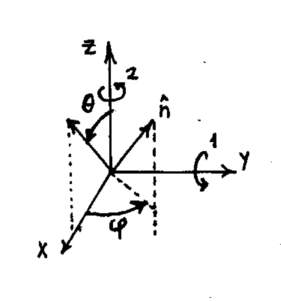
\includegraphics[width=0.25\textwidth]{images/teo2_12.pdf}
	\end{center}
	\caption{.}
\end{figure} 
Necesitamos aplicar $\mathcal{D}(R)=\mathcal{D}(\alpha=\varphi,\beta=\theta,\gamma=0)$
\[
	\Ket{\hat{n}} = \sum_{m,\ell} \mathcal{D} (R) \Ket{\ell,m}\Braket{\ell,m|\hat{z}}
\]
\[
	\Braket{\ell,m'|\hat{n}} = \sum_{m,\ell} \Braket{\ell,m'|\mathcal{D} (R)| \ell,m}\Braket{\ell,m|\hat{z}}
\]
pero como la $\mathcal{D}(R)$ no conecta $\ell$ diferentes, se tiene 
\[
	\Braket{\ell,m'|\hat{n}} = \sum_{m} \mathcal{D}_{m'm}^\ell(R) \Braket{\ell,m|\hat{z}}	
\]
\[
	Y_\ell^{m'*}(\theta,\varphi) = \sum_m \mathcal{D}_{m'm}^\ell(R) Y_\ell^{m*} (\theta=0,\varphi \text{indet})
\]
pero como $\theta=0$ , $Y_\ell^m = 0$  con $m\neq 0$ se tiene 
\[
	\Braket{\ell,m|\hat{z}} = Y_\ell^{m*} (\theta=0,\varphi \text{indet}) \delta_{m0}
\]
\[
	\Braket{\ell,m|\hat{z}} = \sqrt{ \frac{2\ell +1}{4\pi} } \delta_{m0}
\]
\[
	Y_\ell^{m'*}(\theta,\varphi) = \sqrt{ \frac{2\ell +1}{4\pi} }
	\mathcal{D}_{m'0}^\ell (\alpha=\varphi,\beta=\theta,\gamma=0)
\]
la matriz de rotación en este caso es un armónico esférico.

La $\Psi$ tiene la misma simetría que el potencial.

% =================================================================================================
\section{Suma de momentos angulares}
% =================================================================================================

\subsection{Dos momentos de spín $1/2$}

Sean dos estados de spín $1/2$
\[
	\vb{S} = \vb{S}_1 + \vb{S}_2 \equiv \vb{S}_1 \otimes \mathbb{1}_2 + \mathbb{1}_1\otimes \vb{S}_2
\]
en cada espacio valen las relaciones usuales de conmutación 
\[
	[ S_{1/2i},S_{1/2j}] = i\hbar\epsilon_{ijk}S_{1/2k}, \qquad  [S_{1i},S_{2j}] = 0
\]
donde el último indica que operadores de espacios diferentes conmutan.

Un estado general es 
\[
	\Ket{S_1,m_1} \otimes \Ket{S_2,m_2} \equiv \Ket{S_1, S_2;m_1,m_2}
\]
Hay cuatro estados
\[
	\begin{matrix} S_1 \quad S_2 \quad\quad m_1 \quad m_2 \end{matrix}
\]
\[
	\begin{matrix}
	&\Ket{1/2, 1/2 ; \phantom{-}1/2, \phantom{-}1/2} \\
	&\Ket{1/2, 1/2 ; \phantom{-}1/2, -1/2} \\
	&\Ket{1/2, 1/2 ; -1/2, -1/2} \\
	&\Ket{1/2, 1/2 ; -1/2, \phantom{-}1/2}
	\end{matrix}
\]	
\[	
	\begin{matrix} S_1 \quad S_2 \quad\quad S_{1z} \quad S_{2z}  \end{matrix}
\]
que corresponden a los operadores $S_ 1^2, S_2^2, S_{1z}, S_{2z}$ que conmutan (son un CCOC).

Podemos elegir otras base de operadores que comutan que será: $S_ 1^2, S_2^2, S, S_{z}$, de modo que el estado 
general será
\[
	\Ket{S_1, S_2;S,m}
\]
Así tendremos
\[
	\begin{matrix} \qquad\qquad S_1 \quad S_2 \quad S \quad m \end{matrix}
\]
\[
	\begin{matrix}
	\text{Triplete}\begin{cases}	
	&\Ket{1/2, 1/2 \; ; \; 1, \phantom{-}1} \\
	&\Ket{1/2, 1/2 \; ; \; 1, \phantom{-}0} \\
	&\Ket{1/2, 1/2 \; ; \; 1, -1} \\
	\end{cases}
	\\
	\text{Singlete}\begin{cases}
	&\Ket{1/2, 1/2 \; ; \; 0, \phantom{-}0} \\
	\end{cases}		
	\end{matrix}	 
\]	
\[	
	\begin{matrix} \qquad\qquad S_1^2 \quad S_2^2 \quad S^2 \quad S_z  \end{matrix}
\]
y recordemos que $m_1+m_2=m$ y $s_1+s_2=s$
\[
	S^2 = (S_1 + S_2)^2  = S_1^2 + S_2^2 + 2\vb{S}_1\cdot\vb{S}_2 \qquad 
	S^2_z = (S_{1z} + S_{2z})^2  = S_{1z}^2 + S_{2z}^2 + 2S_{1z}\cdot S_{2z}
\]

Dada la repetición de $S_1,D_2$ se suelen identificar a las bases solamente 
\[
	\begin{cases}
	\{ \Ket{m_1,m_2} \} \\
	\{ \Ket{S,m} \}
	\end{cases}
\]
Además la base $\{ \Ket{m_1,m_2}\}$ se puede poner como 
\[
	+ \equiv + 1/2 \qquad\qquad - \equiv - 1/2
\]

\subsection{Cambio entre bases}

Podemos hallar a ojo que 
% \[
% 	\cdot \Ket{++} = \Ket{1,1} \qquad \cdot \Ket{--} = \Ket{1,-1}
% \]
\begin{itemize}
 \item $\Ket{++} = \Ket{1,1}$
 \item $\Ket{--} = \Ket{1,-1}$
\end{itemize}

de manera que la única forma de tener $m=1$ es con los dos spines up y la única forma de tener $m=-1$ es con 
los dos spines down.

Se hallan los otros con el operador de bajada
\[
	S_- \equiv S_{1-} + S_{2-}
\]
y si descompongo $S_-$ en $S_{1-}$ y $S_{2-}$ para operar en $\Braket{s,m}$ se tiene 
\[
	S_- \Ket{++} = S_{1-}\Ket{++} + S_{2-}\Ket{++} = S_{1-}\otimes\mathbb{1}_2\Ket{++} +
	\mathbb{1}_1\otimes S_{2-}\Ket{++} = \hbar\Ket{-+} + \hbar\Ket{+-}
\]
y ahora si opero con $S_-$,
\[
	S_-\Ket{11} = \sqrt{2} \hbar \Ket{10}
\]
\begin{itemize}
	\item $\Ket{10} = \frac{1}{\sqrt{2}}( \Ket{-+} + Ket{+-} ) $
\end{itemize}


Luego
\[
	\Ket{00} = a \Ket{+-} + b\Ket{-+}
\]
y puedo usar ortonormalidad 
\[
	\Braket{10|00} = 0 = \frac{a}{\sqrt{2}} + \frac{b}{\sqrt{2}} \qquad \text{con} \; |a|^2 + |b|^2 = 1
\]
\begin{itemize}
	\item $\displaystyle \Ket{00} = \frac{1}{\sqrt{2}}( \Ket{+-} - \Ket{-+} ) $
\end{itemize}


\section{Teoría formal de suma de momentos angulares}

Sea de sumar dos momentos angulares $J_1, J_2$. Las relaciones de conmutación son
\[
	[J_{1i},J_{1j}] = i\hbar \varepsilon_{ijk}J_{1k} \qquad 
	[J_{2i},J_{2j}] = i\hbar \varepsilon_{ijk}J_{2k} \qquad
	[J_{1k},J_{2l}] = 0
\]
\[
	\vb{J} = \vb{J}_1 \otimes \mathbb{1}_2 + \mathbb{1}_1\otimes \vb{J}_2 \equiv \vb{J}_1 + \vb{J}_2
\]
\[
	[J_i, J_j] = i\hbar\epsilon_{ijk}J_k
\]

El momento total \vb{J} cumple que 
\[
	J^2 =  J_1^2 + J_2^2 + 2J_1J_2 \qquad 
	J^2 =  J_1^2 + J_2^2 + 2J_{1z}J_{2z} + J_{1+}J_{2-} + J_{1-}J_{2+}
\]
donde vemos que 
\[
	[J^2_{1/2},J^2] = 0 \qquad [J_z,J^2] = 0 \qquad [J^2_{1/2},J_{1/2,z,+,-}] = 0
\]
pero 
\[
	[ J^2 , J_{1z}] \neq 0  \qquad \qquad [ J^2 , J_{2z}] \neq 0
\]

Esto deja dos opciones para elegir un CCOC

\begin{center}
\begin{tabular}{|c|c|}
\hline 
$J_1^2, J_2^2, J_{1z}, J_{2z}$ & $J_1^2, J_2^2, J^2, J_{z}$ \\
& \\
$\Ket{j_1,j_2;m_1,m_2}$ & $\Ket{j_1,j_2;j,m}$ \\
& \\
base desacoplada & base acoplada \\
\hline
\end{tabular}
\end{center}

Se puede pasar de una base a otra con una identidad $\mathbb{1}$ apropiada
\[
	\Ket{j_1,j_2;j,m} = \sum_{m_1,m_2} \Ket{j_1,j_2;m_1,m_2}\Braket{j_1,j_2;m_1,m_2|j_1,j_2;j,m}
\]
\[
	1. \; \Ket{j_1,j_2;j,m} = \sum_{m_1,m_2} C_{m_1m_2}^j \Ket{j_1,j_2;m_1,m_2}
\]
con $-j_1 \leq m_1 \leq j_1$ y  $-j_2 \leq m_2 \leq j_2$
\[
	\Ket{j_1,j_2;m_1,m_2} = \sum_{j,m} \Ket{j_1,j_2;j,m}\Braket{j_1,j_2;j,m|j_1,j_2;m_1,m_2}
\]
\[
	2. \; \Ket{j_1,j_2;m_1,m_2} = \sum_{j,m} C_{m_1m_2}^{j*}\Ket{j_1,j_2;j,m}
\]
con $-j \leq m \leq j$ y con $j\to\infty$.

Donde los $C_{m_1 m_2}^j$ son los coeficientes de Clebsh-Gordan. En 2 la $\sum$ sería en $j\to\infty$, pero veamos la 
relacion que hace algunos $C_{m_1 m_2}^j=0$. Ante todo abreviaremos suprimiendo los índices $j_1,j_2$ con lo cual 
\[
	C_{m_1m_2}^{j} = \Braket{m_1,m_2|j,m}
\]

\subsection{Restricciones para la no nulidad de los coeficientes}

\[
	(J_{z} - J_{1z} - J_{2z})\Ket{j,m} = (m\hbar - J_{1z} - J_{2z})\Ket{j,m} = 0
\]
\[
	\Braket{m_1,m_2|(J_{z} - J_{1z} - J_{2z})|j,m}= 0 \qquad \qquad 
	\hbar(m-m_1-m_2)\Braket{m_1,m_2|j,m} = 0
\]
entonces
\[
	\Braket{m_1,m_2| j,m} \neq 0 \iff m = m_1 + m_2
\]

A su vez, en la suma de $J_1$ y $J_2$ resultan los $j$ acotados por una desigualdad triangular 
\[
	|j_1 - j_2| \leq j \leq j_1 + j_2
\]

Asimismo los $C_{m_1 m_2}^j$ se toman reales, entonces 
\[
	C_{m_1m_2}^{j*} = C_{m_1m_2}^{j}
\]
y juntando todo se tiene 
\[
	\Braket{m_1,m_2|j,m} \neq 0	\iff  m = m_1 + m_2,
\]
o lo que es equivalente
\[
	\Braket{j,m|m_1,m_2} \iff |j_1 - j_2| \leq j \leq j_1 + j_2
\]

Ambas bases tienen la misma dimensión
\[
	\sum = (2j_1 + 1)(2j_2 + 1)
\]

Recordemos que cada $j$ tiene $2j+1$ estados posibles (los $m$ correspondientes a cada $j$) ($|m|\leq j$). Si 
sumamos $j_1=1, j_2=3/2$ tendremos 
\[
	\text{dim} =  2 \oplus 4 \oplus 6 = 3 \otimes 4 = 12
\]
\[
	j = 1/2, 3/2, 5/2 \qquad m_1 = -1,0,1
\]
\[
	j = -5/2,-3/2,-1/2,1/2, 3/2, 5/2 \qquad m_2 = -3/2,-1/2,1/2,3/2
\]

Podemos ver a ojo que 
\[
	\Ket{j=5/2,m=5/2} = \Ket{m_1=1,m_2=3/2}
\]
\[
	\Ket{j=5/2,m=-5/2} = \Ket{m_1=-1,m_2=-3/2}
\]
luego con el $J_=, J_-$ podemos construirnos los siguientes (utilizando ortonormalidad)
\[
	\Braket{j',m'|j,m} = \delta_{j'j}\delta_{m'm}
\]
\[
	\sum_{m_1,m_2} \Braket{j',m'|m_1,m_2}\Braket{m_1,m_2|j,m} = \delta_{j'j}\delta_{m'm}
\]
\[
	\sum_{m_1,m_2} \Braket{m_1,m_2|j,m}^2 = 1
\]
siendo esto último la ortonormalidad.

\subsection{Relación de recurrencia}

\[
	J_\pm \ket{j,m} = ( J_{1\pm} + J_{2\pm} ) \sum_{m_1',m_2'} \Ket{m_1',m_2'}\Braket{m_1',m_2'|j,m}
\]
\[
	\sqrt{(j\mp m)(j\pm m + 1)} \ket{j,m\pm 1} = \sum_{m_1',m_2'}\Braket{m_1',m_2'|j,m}  
	( J_{1\pm}\Ket{m_1',m_2'} + J_{2\pm}\Ket{m_1',m_2'} ) 
\]
y metiendo un bra $\Bra{m_1,m_2}$ se llega a la relación de recurrencia
\begin{multline*}
	\sqrt{(j\mp m)(j\pm m + 1)} \Braket{m_1,m_2|j,m\pm 1} =
	\sqrt{(j_1 \mp m_1 + 1 )(j_1 \pm m_1)} \Braket{m_1 \mp 1 ,m_2|j,m}  + \\
	\sqrt{(j_2 \mp m_2 + 1 )(j_2 \pm m_2)}  \Braket{m_1,m_2 \mp 1| j,m } 
\end{multline*}


\subsection{Suma de \vb{L} y \vb{S}}

Sea suma \vb{L} y \vb{S}, entonces 
\[
	j_1 = l \qquad j_2 = S= 1/2 \quad m_1=m_l \quad m_2=m_s = \pm 1/2
\]
\[
	|l - 1/2| \leq j \leq l + 1/2  \qquad j=\begin{cases} l-1/2 \\ l+1/2\end{cases}
\]
\[
	m = m_l \pm 1/2 \qquad m_l = m + 1/2 , m- 1/2 \qquad m_S = 1/2, -1/2
\]
y luego dim=$(2l+1)\otimes 2 =) 4l+2$.
Habrá sólo cuatro $C_{m_1 m_2}^j$ no nulos, que serán 
\[
	\Braket{ m + 1/2, -1/2 | l - 1/2, m }
\]
\[
	\Braket{ m + 1/2, -1/2 | l + 1/2, m }
\]
\[
	\Braket{ m - 1/2, 1/2 | l - 1/2, m }
\]
\[
	\Braket{ m - 1/2, 1/2 | l + 1/2, m }
\]
donde vemos que los coeficientes linkean sólo los estados con $j=\ell-1/2$ y $j=\ell+1/2$ y podemos construir 
una matriz de $2\times 2$ para este caso.

Esto tórnase práctico para acoplamiento spin-órbita 
\[
	\vb{L}\cdot\vb{S} = \frac{1}{2}(J^2 - L^2 - S^2)
\]
\[
	\vb{L}\cdot\vb{S} \Ket{l,s;j,m} =  \frac{1}{2}\left( j(j+1)\hbar^2 - 
		l(l+1)\hbar^2 - s(s+1/2)\hbar^2 \right) \Ket{l,s;j,m}
\]
\[
	= \frac{1}{2}\left( j(j+1) - l(l+1) - 3/4 \right) \hbar^2 \Ket{l,s;j,m}
\]
\[
	\vb{L}\cdot\vb{S} \Ket{l,s;j,m} = \begin{cases} 
		\displaystyle \frac{l\hbar^2}{2} \Ket{l,s;j,m} \quad \text{si} \; j=l+1/2\\ 
		\\
		\displaystyle -\frac{(l+1)\hbar^2}{2}\Ket{l,s;j,m} \quad \text{si} \; j=l-1/2
	\end{cases}
\]

\section{Operadores vectoriales}

Queremos analizar como transforma un operador vectorial $\hat{v}$ bajo rotaciones en mecánica cuántica.
En mecánica clásica,
\[
	V_i = R_{ij} V_j \qquad \text{con} \; R \; \text{matriz diagonal}
\]
En mecánica cuántica tenemos que al rotar
\[
	\Ket{\alpha}_R = \mathcal{D}(R)\Ket{\alpha}
\]
Pediremos entonces que $\Braket{V}$ transforme como un vector y eso lleva a que 
\[
	\Braket{\alpha|V_i|\alpha}_R = \Braket{\alpha|\mathcal{D}^\dagger(R)V_i\mathcal{D}(R)|\alpha} =
	R_{ij} \Braket{\alpha|V_j|\alpha}
\]
\[
	\mathcal{D}(R)^\dagger V_i \mathcal{D}(R) = R_{ij}V_j \qquad (º)
\]
y calculando la expresión anterior (1) llegamos a que debe valer
\[
	[V_i,J_j] =  i\hbar \varepsilon_{ijR}V_R
\]
que es la manera de transformar de un operador vectorial. Podemos probar un caso simple de una rotación 
infinitesimal en $\hat{z}$ y ver que vale.


\section{Operadores tensoriales}

En mecánica clásica 
\[
	T_{ij} = R_{ii'} R_{jj'} T_{i' j'}
\]
que es un tensor de rango dos. Esto es un \underline{tensor cartesiano}. Su problema es que \underline{no es 
irreducible}, entonces puede descomponerse en objetos que transforman diferente ante rotaciones. Sea la díada 
$U_iV_j$, tensor de rango dos, que puede escribirse como 
\[
	UV = \frac{1}{3}\vb{U}\cdot\vb{V}\delta_{ij} + \frac{1}{2}\left( U_iV_j - U_jV_i \right) +
	\left[ \frac{1}{2}\left( U_iV_j + U_jV_i \right) - \frac{1}{3}\vb{U}\cdot\vb{V}\delta_{ij}\right]
\]
Hemos reducido el tensor cartesiano en tensores irreducibles. Podemos asociar esta descomposición con las 
multiplicidades de objetos con momento angular $\ell=0, \ell=1, \ell=2$
\[
	\text{escalar} \longrightarrow \ell=0 \; \text{singlete (un elemento independiente) }
\]
\[
	\text{vector} \longrightarrow \ell=1 \; \text{triplete (tres elementos independientes)}
\]
\[
	\text{tensor de traza nula} \longrightarrow \ell=2 \; \text{quintuplete (cinco elementos 
independientes)}
\]

Se define 
\[
	T^{(k)}_q \qquad \text{tensor esférico de rango $k$ y número magnético $q$}
\]
Un tensor esférico transforma como 
\[
	\mathcal{D}(R) T_{q'}^{(k)} \mathcal{D}(R)^\dagger = \mathcal{D}(R) T_{q'}^{(k)}  \qquad (2)
\]
Tendremos 
\[
	T^{(0)}_0 \quad \text{(escalar) tensor esférico de rango 0 ($\ell=0$)}
\]
\[
	(T^{(1)}_1,T^{(1)}_0,T^{(1)}_{-1}) \quad \text{(vector) tensor esférico de rango 1 ($\ell=1$)}
\]

En muchos casos se puede escribir un tensor esférico como armónico esférico 
\[
	Y_\ell^{m}(\theta,\varphi) = Y_\ell^{m}(\hat{n}) \; \longrightarrow 
	\overbrace{ \phantom{.}\hat{n} \longrightarrow \vec{v}\phantom{.}}^{\text{paso}} \quad
	Y_\ell^m(\vec{v}) \equiv Y_k^q(\vec{v}) = T_q^{(k)}
\]
\[
	\hat{n} = (n_x,n_y,n_z) = \left( \frac{x}{r}, \frac{y}{r}, \frac{z}{r} \right) \quad 
	\longrightarrow \quad \vb{v} = (rn_x,rn_y,rn_z)
\]
\[
	\hat{n} = ( \cos(\phi)\sin(\theta), \sin(\phi)\sin(\theta), \cos(\theta))
\]
\[
	Y_1^0 = \sqrt{\frac{3}{4\pi}}n_z \quad \longrightarrow \quad T_1^0 = \sqrt{\frac{3}{4\pi}}V_z
\]
\[
	Y_1^{\pm 1} = \mp \sqrt{\frac{3}{4\pi}} \frac{n_x \pm i n_y}{\sqrt{2}} \quad \longrightarrow
	T_{\pm 1}^{(1)} = \mp \sqrt{\frac{3}{4\pi}} \frac{V_x \pm i V_y}{\sqrt{2}}
\]
Calculando en (2), cosa que podemos hacer para, por ejemplo, una rotación infinitesimal, llegamos a las 
relaciones de conmutación para tensores.
\[
	[ J_z, T_q^{(k)} ] = \hbar q T_q^{(k)} \qquad 
	[J_{\pm},T_q^{(k)}] = \hbar \sqrt{(k\mp 1)(k\pm q + 1)} T_{q\pm 1}^{(k)}
\]


% \bibliographystyle{CBFT-apa-good}	% (uses file "apa-good.bst")
% \bibliography{CBFT.Referencias} % La base de datos bibliográfica

\end{document}
